\documentclass[a4paper, 12pt]{article}

\usepackage[portuges]{babel}
\usepackage[utf8]{inputenc}
\usepackage{amsmath}
\usepackage{indentfirst}
\usepackage{graphicx}
\usepackage{multicol,lipsum}

\begin{document}

\begin{titlepage}
    \begin{center}

        \begin{figure}[!ht]
            \centering
            
\includegraphics[width=10cm]{images/IST.png}
        \end{figure}

        \Huge{Instituto Superior Técnico}\\
        \large{LEEC}\\
        \large{Sinais e Sistemas}\\
        \vspace{15pt}
        \vspace{95pt}
        \textbf{\LARGE{Relatório Laboratório Sinais e Sistemas}}\\
        \vspace{3,5cm}
    \end{center}

    \begin{flushleft}
        \begin{tabbing}
            Aluno: Henrique Machado 103202 \\
            Aluno: Miguel Neves 103462 \\
            Grupo: 79
        \end{tabbing}
    \end{flushleft}
    \vspace{1cm}

    \begin{center}
        \vspace{\fill}
        Janeiro\\
        2023
    \end{center}
\end{titlepage}
%%%%%%%%%%%%%%%%%%%%%%%%%%%%%%%%%%%%%%%%%%%%%%%%%%%%%%%%%%%
% % % % % % % % % % % % % % % % % % % % % % % % % %
\newpage
\tableofcontents
\thispagestyle{empty}
\newpage
\pagenumbering{arabic}
% % % % % % % % % % % % % % % % % % % % % % % % % % %
\section{Sinais Sinusoidais}
\begin{itemize}
    \item \textbf{Q1:} As sinusoidais com frequência mais altas correspondem aos sons mais agudos, inversamente, as sinusoidais com frequência mais baixa correspondem aos sons mais graves.
    \item \textbf{Q2:} A frequência minima que nós conseguimos ouvir foi $55hz$ e a frequência máxima que conseguimos ouvir foi $18000hz$.
\end{itemize}
% % % % % % % % % % % % % % % % % % % % % % % % % % %
\vspace{15px}
\section{Notas Musicais}
\begin{itemize}
    \item \textbf{Q3:}
          \begin{enumerate}
              \item[] Mi$_4$: $329.63hz$
              \item[] Fá$_4^\#$: $370.00hz$
              \item[] Sol$_4$: $392.00hz$
              \item[] Si$_4$: $493.89hz$
              \item[] Dó$_5$: $554.37hz$
          \end{enumerate}
\end{itemize}
% % % % % % % % % % % % % % % % % % % % % % % % % % %
\vspace{15px}
\section{Impulso e Degrau Unitários}
\begin{itemize}
    \item \textbf{Q4:} Com base na definição de degrau unitário, $u(at+b)$ pode ser escrito como $u(\pm t - t_0)$ uma vez que: $t_0 = \frac{b}{|a|}$, onde temos que
          \[ \begin{cases}
                  a > 0, & t > 0 \\
                  a < 0, & t < 0
              \end{cases} \]
          Caso $a < 0$, verifica-se uma inversão no tempo do gráfico de $u(t)$.
          \newpage
    \item \textbf{Q5:} $\delta(at) = \frac{1}{\Delta}[u(at) - u(at - \Delta)]$ e $\delta(at) = \underset{{\Delta\to0}}{\lim}\delta_\Delta(at)$, com $a > 0$\vspace{15px}\\
          Para $\delta(t)$\hspace{150px}Para$\delta(at)$\\
          \begin{figure}[!ht]
              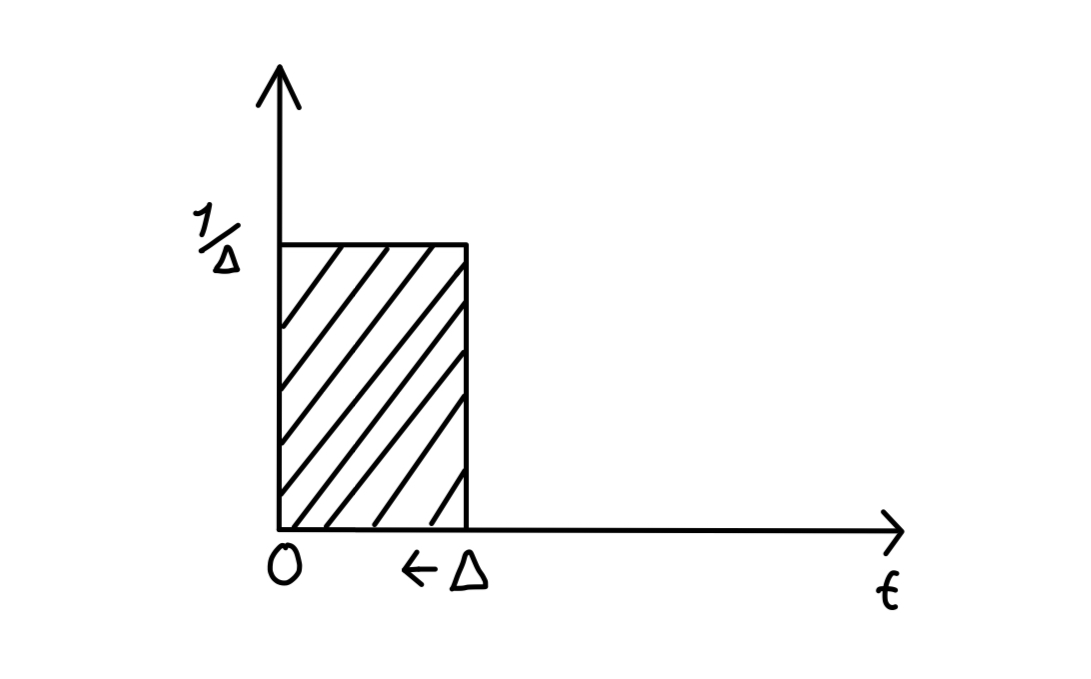
\includegraphics[width=6cm]{images/Graf1.png}
              \hspace{10px}
              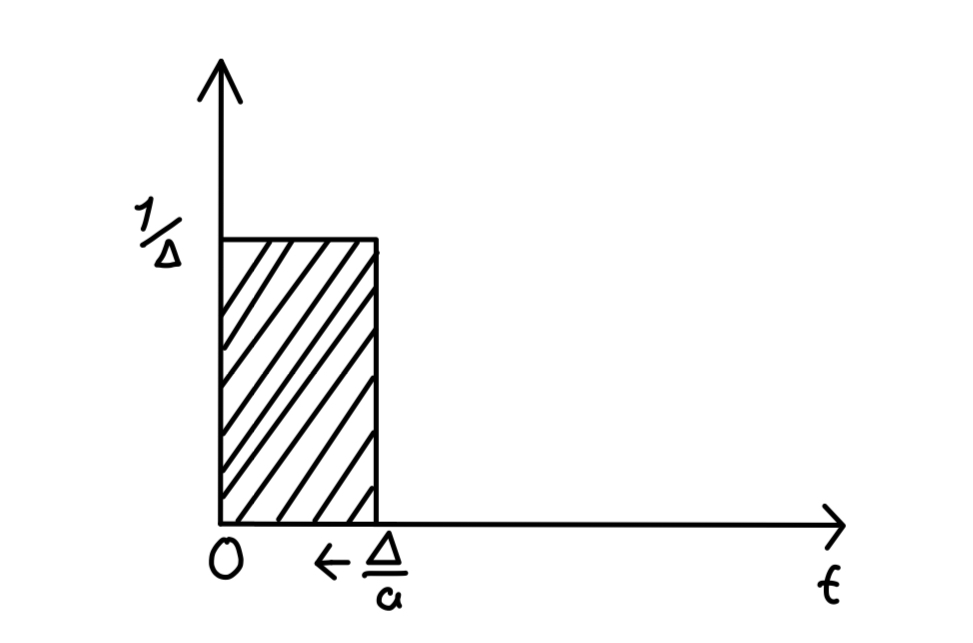
\includegraphics[width=6cm]{images/Graf2.png}
              \vspace{-10px}
              \caption{Comparação entre os gráficos entre $\delta(t) \textrm{ e } \delta(at)$}
          \end{figure}\\
          Área $ = \frac{1}{\Delta}\times\Delta = 1$\hspace{100px}Área $= \frac{1}{\Delta} \times \frac{\Delta}{a} = \frac{1}{a}$\vspace{15px}\\
          Logo, $\delta(at) = \frac{1}{a}\delta(t)$, com $a > 0$.\vspace{5px}
    \item \textbf{Q6:} Não se verifica nenhuma mudança no gráfico de $\delta(at)$ em relação ao gráfico de $\delta(t)$. No entanto, pelo que foi concluído previamente, o que deveria acontecer seria uma redução da área do impulso devido ao produto pelo termo $\frac{1}{a}$ (sendo $a > 1$) transformação esta que não é visível no visor.
\end{itemize}
\newpage
% % % % % % % % % % % % % % % % % % % % % % % % % % %
\section{Sistemas}
\begin{itemize}
    \item \textbf{Q7:} O sistema apresentado é linear:
          \[x_1(t) \to y_1(t) = x_1(t) + 0.5x_1(t - 0.25)\]
          \[x_2(t) \to y_2(t) = x_2(t) + 0.5x_2(t - 0.25)\]
          $x_3(t) \to$ Combinação linear de $x_1(t)$ e $x_2(t) : x_3(t) = ax_1(t) + bx_2(t)$\vspace{-5px}
          \[y_3(t) = x_3(t) + 0.5x_3(t + 0.25)\]
          \[= ax_1(t) + bx_2(t  ) + 0.5(ax_1(t - 0.25) + bx_2(t - 0.25))\]
          \[= ax_1(t) + bx_2(t) + 0.5ax_1(t - 0.25) + 0.5bx_2(t - 0.25)\]
          \[= a(x_1(t) + 0.5x_1(t - 0.25)) + b(x_2(t) + 0.5x_2(t- 0.25))\]
          \hspace{105px}$= ay_1(t) + by_2(t) \to$ é linear.\\\vspace{-9px}
          E é invariante no tempo:
          \[y_1(t) = x_1(t) + 0.5x_1(t - 0.25)\]
          \[x_2(t) = x_1(t - t_0) \to y_2(t) = x_2(t) + 0.5x_2(t - 0.25)\]
          \hspace{184px}$= x_1(t - t_0) + 0.5x_1(t- t_0 - 0.25)$
          \[y_1(t - t_0) = x_1(t - t_0) + 0.5x_1(t - t_0 - 0.25)\]
          \hspace{57px}logo $y_2(t) = y_1(t - t_0) \to$ é invariante no tempo.
    \item \textbf{Q8:} Resposta do sistema ao impulso unitário: $\delta(t)y(t) = \delta(t) + 0.5\delta(t - 0.25)$
          \begin{figure}[!ht]
              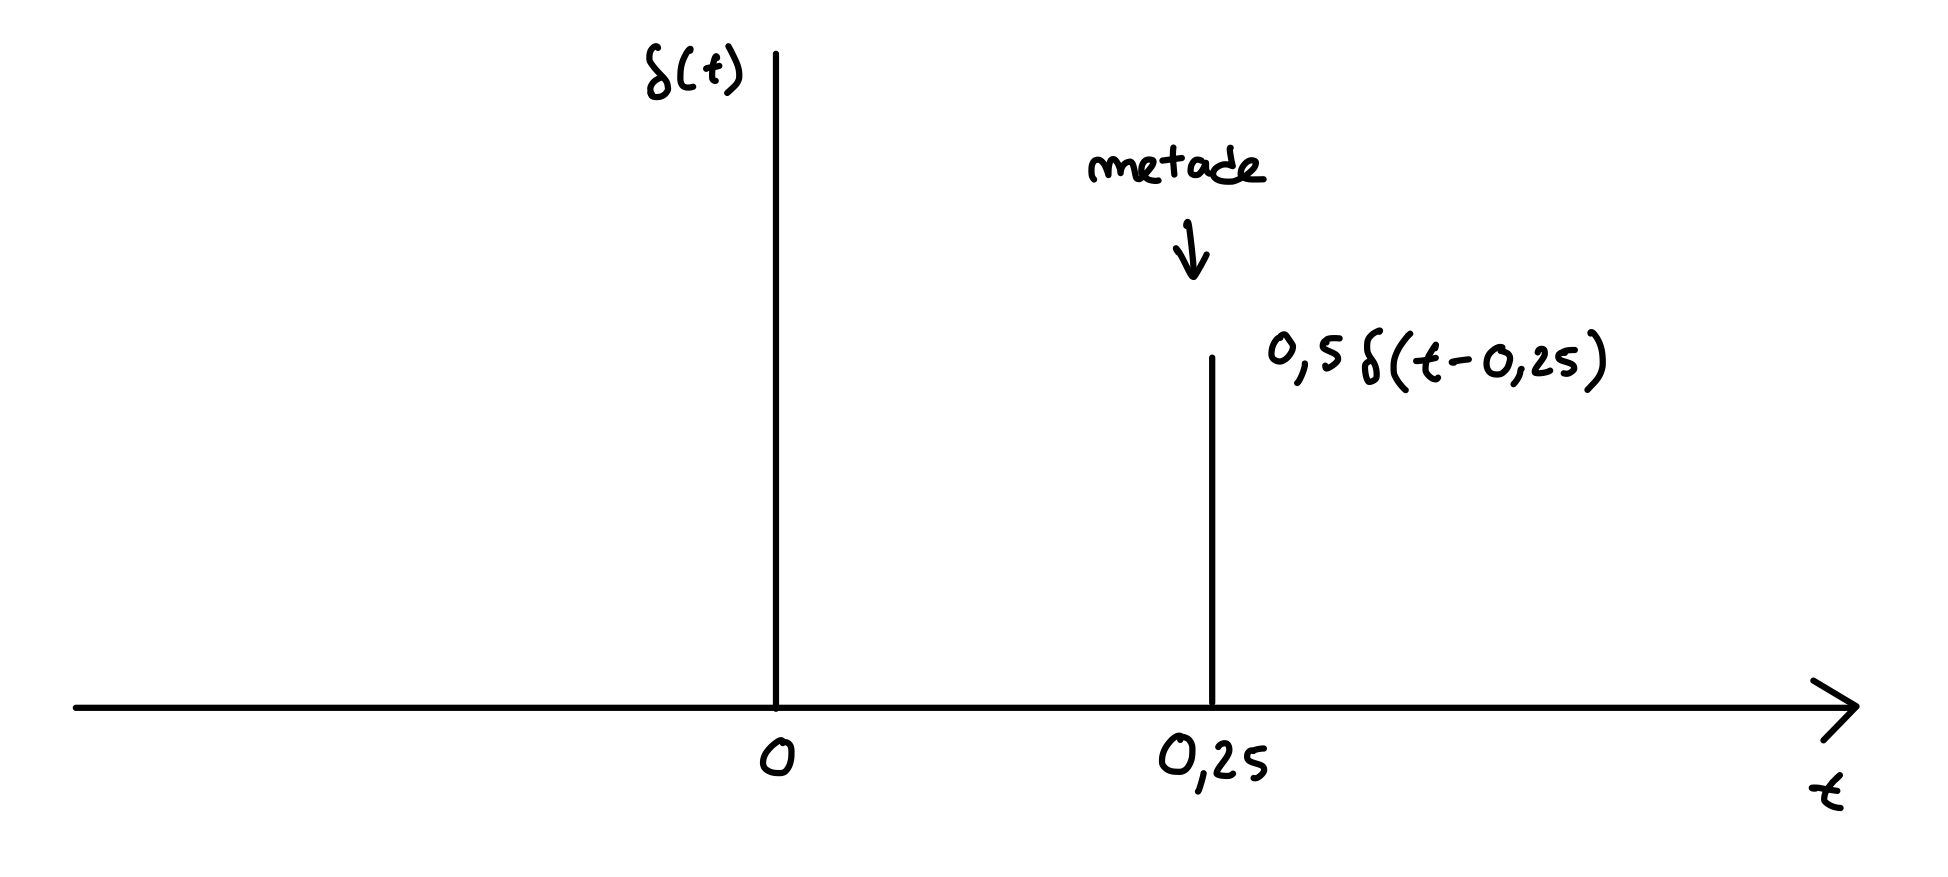
\includegraphics[width=12cm]{images/Graf3.png}
              \vspace{-15px}
              \caption{Visualização dos gráficos}
          \end{figure}
    \item \textbf{Q9:} O sistema apresentado $(y(t))$ possui memória visto que não depende apenas do valor de $x(t)$ mas sim de $x(t)$ e de $(t - 0.25)$. Para além disso é um sistema causal uma vez que o seu output depende apenas dos valores do presente $x(t)$ e do passado $x(t - 0.25)$. Em relação à sua estabilidade, pode-se afirmar que é um sistema estável, visto que não é possível encontrar nenhum input limitado que provocasse um output não limitado:\\
          Sendo $a, b$ números arbitrários que verificam as condições
          \[\begin{cases}
                  |x(t)| < a \\
                  |x(t - 0.25)| < b
              \end{cases}\]
          Então: $-a - 0.5b < y(t) < at + 0.5b$, o que representa um output limitado.
    \item \textbf{Q10:} O efeito produzido pelo sistema é um eco (prolongamento do som).
    \item \textbf{Q11:} $x_2(t) = \cos(44t)$, que pode ser escrito como
          \[x_2(t) = \frac{1}{2}e^{j44t} + \frac{1}{2}e^{-j44t}\]
          $y_2(t) = x_2(t) + 0.5x_2(t - 0.25) =$
          \[= \frac{1}{2}e^{j44t} + \frac{1}{2}e^{-j44t} + \frac{1}{2}\left(\frac{1}{2}e^{j44t - 0.25}+\frac{1}{2}e^{-j44t + 0.25}\right)\]
          \[= \frac{1}{2}e^{j44t} + \frac{1}{2}e^{-j44t} + \frac{1}{4}e^{j44t - 11} + \frac{1}{4}e^{-j44t + 11}\]
          \[= \frac{1}{2}e^{j44t} + \frac{1}{2}e^{-j44t} + \frac{1}{4e^{11}}e^{j44t} + \frac{e^{11}}{4}e^{-j44t}\]
          \[= \frac{2e^{11} + 1}{4e^{11}}e^{j44t} + \frac{2+e^{11}}{4}e^{-j44t}\]
          \newpage
    \item \textbf{Q12:} Para avaliarmos estas propriedades deste sistema, testamos o seu comportamento com vários sinais de input.\vspace{10px}\\
          Para testar a linearidade, testamos com $x_1(t) = u(t)$ e com $x_2(t) = 2tu(t)$. Ao analisarmos os gráficos de saída obtidos, não se verificou que $y_0(t) = 2ty_1(t)$, logo o sistema não é linear.\vspace{10px}\\
          Em relação à invariância no tempo, utilizámos o mesmo input $x_1(t) = u(t)$, mas agora um $x_2(t) = u(t - 1)$. Para o sistema ser invariante no tempo, o gráfico obtido de saída de $y_2(t)$ deveria traduzir-se numa translação do gráfico de $y_1(t)$, algo que não acontece. Assim, conclui-se que o sistema não é variante no tempo.\vspace{10px}\\
          Para testar a memória, utilizámos os inputs $x_1(t) = 0$ e $x_2(t) = \delta(t)$. Apenas em $t = 0$, os valores dos sinais de entrada seriam diferentes na hipótese do sistema não ter memória. No entanto verificam-se mais instantes em que isso acontece, logo o sistema tem memória.\vspace{10px}\\
          No que diz respeito à causalidade, por mais testes que realizássemos para vários sinais de entrada, nunca seria possível concluir nada pois seria necessário testar toda a infinidade de entradas possíveis. No entanto para os testes que efetuamos, aparenta ser um sinal causal.\vspace{10px}\\
          Por último, testamos o sistema com alguns sinais de entrada limitados, sendo o resultado obtido também limitado. Contudo, tal como a causalidade, não podemos ter a certeza porque o sistema tem de ter este comportamento para todos os inputs possíveis.
\end{itemize}
\newpage
% % % % % % % % % % % % % % % % % % % % % % % % % % %
\section{Série de Fourier}
\begin{itemize}
    \item \textbf{Q13:} $w_0 = \frac{2\pi}{T} = \frac{2\pi}{0.4} = 5\pi$\hspace{50px}$T = 0.4$
          \[a_0 = \frac{1}{T}\int_{T}x(t)dt = \frac{1}{0.4} \times 1.2 = \frac{12}{4} = 3\hspace{15px} \vspace{10px}\]
          Utilizando as propriedades da série de Fourier:\vspace{10px}
          \[a_k = \frac{1}{T}\int_{-T_1}^{T_1}e^{-jkw_{0}t}dt = \frac{\sin(kw_{0}T_1)}{k\pi} = \frac{\sin(k \times 5\pi \times 0.2)}{k\pi} = \frac{\sin(k\pi)}{k\pi}\]
          Propriedade do deslocamento $\to b_k = a_{k}e^{-jk(5\pi)0.1} = a_{k}e^{-jk0.5\pi}$\\
          Existe um offset que provoca um deslocamento do sinal para cima, que afeta apenas $a_0$
          \[b_k =
              \begin{cases}
                  0, \textrm{ }k\neq0 \\
                  4, \textrm{ }k = 0
              \end{cases}
              \hspace{15px}
              e_k =
              \begin{cases}
                  a_{k}e^{-jk0.5\pi}, \textrm{ }k\neq0 \\
                  a_{0} + 4, \textrm{ }k = 0
              \end{cases}\]
          Propriedade da derivada:\vspace{10px}\\
          Para $k\neq0$:
          \[e_k = jk(5\pi)dk \Leftrightarrow d_k = \frac{e_k}{5\pi jk} \Leftrightarrow d_k = \frac{a_{k}e^{-jk0.5\pi}}{5\pi jk} \Leftrightarrow d_k = \frac{\sin(k\pi)e^{-jk0.5\pi}}{5\pi^{2}k^{2}j}\]
    \item \textbf{Q14:} \[x_N(t) = \sum_{k = -N}^{N} a_{k}e^{jkw_{0}t} = \sum_{k = -\inf}^{-1}a_{k}e^{jkw_{0}t} + a_{0} + \sum_{k=1}^{+\inf}a_{k}e^{jkw_{0}t}\]
          \[= \sum_{k = -\inf}^{-1}a_{k}(\cos(kw_{0}t) - j\sin(kw_{0}t)) + a_{0} + \sum_{k = 1}^{+\inf}a_{k}(\cos(kw_{0}t) + j\sin(kw_{0}t))\]
          \[= a_{0} + \sum_{k=1}^{+\inf}a_{k}\cos(\varphi_{k})\cos(kw_{0}t) - a_{k}\sin(\varphi_{k})\sin(kw_{0}t)\]
          \[= a_{0} + \sum_{k=1}^{+\inf}a_{k}\cos(kw_{0}t + \varphi_{k})\]
          Sendo $a = a_{k}\cos(\varphi_k)\hspace{15px}b=-a_k\sin(\varphi_{k})$, então:
          \[A_{k} = \sqrt{(a^{2}+b^{2})} \textrm{ e } \varphi_{k} = \arctan(-\frac{b}{a}), A_0 = a_0\]
    \item \textbf{Q15:} $A_0 = a_0 = 0.75 + 0.9 = 1.65$
    \item \textbf{Q16:} A sobreposição destes sinais da série truncada para os vários valores de N forma o sinal original da série de Fourier, o que é o esperado acontecer, uma vez que estamos a unir as várias harmónica. Quantos mais sinais $x_n(t)$ utilizarmos, mais parecido será este gráfico com o sinal original.
    \item \textbf{Q17:} Os gráficos da parte real das transformadas de Fourier dos sinais $x_n(t)$ assemelham-se aos gráficos dos transformadas de Fourier de, por exemplo, uma onda quadrada já que estes sinais $x_n$ são sinais simples.
\end{itemize}
\newpage
% % % % % % % % % % % % % % % % % % % % % % % % % % %
\section{Resposta em Frequência}
\begin{itemize}
    \item \textbf{Q18:} Para determinar o módulo e o argumento da resposta em\\
          frequência do sistema $H(jw)$ para cada valor de $w$, necessitamos de medir experimentalmente no sinal de saída $y(t)$ a amplitude e a fase da frequência $w$.\\
          Com esses valores conseguimos calcular a transformada de Fourier de $y(t)$ a partir da fórmula:
          \[Y(jw) = \int y(t)e^{-jwt}dt\]
          Com isso conseguimos calcular o módulo de $H(jw)$ a partir da fórmula:
          \[ |H(jw)| = \frac{ |Y(jw)| }{ |X(jw)| }\]
          Sendo $X(jw)$a transformada de Fourier de $x(t)$.\\
          O argumento da resposta em frequência do sistema $H(jw)$ é calculado a partir da fórmula:
          \[\angle H(jw) = \angle Y(jw) - \angle X(jw)\]
    \item \textbf{Q19:} Para calcular o módulo da resposta em frequências do sistema3 usaremos a fórmula
          \[ |H(jw)| = \frac{ |Y(jw)| }{ |X(jw)| }\]
          em que $|Y(jw)|$ é a amplitude do sinal de saída e $|X(jw)|$ é a amplitude do sinal de entrada dado por $\cos(wt)$.\vspace{15px}
          \[w = 0, |Y(jw)| = 1 \textrm{ e } |X(jw)| = 1, \textrm{ logo } |H(jw)| = \frac{1}{1} = 1\]
          \[w = 1, |Y(jw)| = 0.933 \textrm{ e } |X(jw)| = 1, \textrm{ logo } |H(jw)| = \frac{0.933}{1} = 0.933\]
          \[w = 3, |Y(jw)| = 0.657 \textrm{ e } |X(jw)| = 3, \textrm{ logo } |H(jw)| = \frac{0.657}{3} = 0.219\]
          \[w = 5, |Y(jw)| = 0.463 \textrm{ e } |X(jw)| = 5, \textrm{ logo } |H(jw)| = \frac{0.463}{5} = 0.0926\]
          \[w = 10, |Y(jw)| = 0.252 \textrm{ e } |X(jw)| = 10, \textrm{ logo } |H(jw)| = \frac{0.252}{10} = 0.0252\]
          \[w = 20, |Y(jw)| = 0.130 \textrm{ e } |X(jw)| = 20, \textrm{ logo } |H(jw)| = \frac{0.130}{20} = 0.0065\]
          \[w = 50, |Y(jw)| = 0.065 \textrm{ e } |X(jw)| = 50, \textrm{ logo } |H(jw)| = \frac{0.065}{50} = 0.0013\]
    \item \textbf{Q20:}
          \begin{figure}[!ht]
              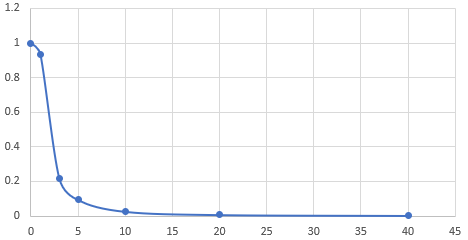
\includegraphics[width = 13.5cm]{images/Graf4.png}
              \vspace{-10px}
              \caption{Gráfico do módulo da resposta em frequência}
          \end{figure}
          \\Interpretando o gráfico conseguimos ver que é um filtro passa baixo, pois com as frequênciasmais baixas o módulo é maior. Este filtro não é ideal pois exibe as características de transmissão com distorção.
    \item \textbf{Q21:} A equação diferencial a que obedece o sistema é:
          \[\tau\frac{dy(t)}{dt} + y(t) = x(t)\]
          uma vez que se trata de um sistema de\\
          primeira ordem, $RC$.\\
          Sendo $\tau>0$ e $x(t) = e^{jwt}: \frac{\tau dy(t)}{dt} + y(t) = x(t)$\\
          Utilizando os propriedades da transformada da série de Fourier (Propriedade da derivada e linearidade):
          \[\Leftrightarrow \tau jwY(jw) + Y(jw) = X(jw)\Leftrightarrow\]
          \[\Leftrightarrow \frac{\tau jwY(jw)}{X(jw)} + \frac{Y(jw)}{X(jw)} = 1 \Leftrightarrow \tau jwH(jw) + H(jw) = 1\]
          \[\Leftrightarrow H(jw)(\tau jw + 1) = 1\]
          \[\Leftrightarrow H(jw) = \frac{1}{\tau jw + 1} \textrm{, Sendo } \tau = RC, H(jw) = \frac{1}{RCjw + 1}\]
          Sendo a resposta do circuito ao impulso unitário $\delta(t)$ dada por $h(t)$
          \[L\delta(\tau) = 1\]
          \[y(t) = \frac{\frac{1}{\tau}}{s + \frac{1}{\tau}} \textrm{ e } x(t) = L^{-1}\{y(t)\} = \frac{1}{\tau}e^{-\frac{\tau}{t}}\]
          \[\textrm{Logo, } h(t) = x(t)\times u(t) = \frac{1}{\tau}e^{-\frac{\tau}{t}} \times u(t) = \frac{1}{RC}e^{-\frac{t}{RC}}u(t)\]
          \[ |H(jw)| = \left|\frac{1}{RCjw + 1}\right| = \frac{|1|}{|RCjw +1|} = \frac{1}{\sqrt{{(RCjw)}^{2} + 1}}\]
          Para calcularmos o $\angle H(jw)$, podemos apenas calcular graficamente o desfazamento do sinal de entrada $x(t)$ com o sinal de saída $y(t)$:
          \[\angle H(jw) = \Delta s \times w \textrm{ , sendo } \Delta s \textrm{ o desfazamento.}\]
          \[\textrm{Ou de outra forma, } \angle H(jw) = -\arctan(wRC)\]
    \item \textbf{Q22:}
          \[H(jw) = \frac{1}{RCjw + 1} \Leftrightarrow H(jw)(RCjw + 1) = 1\]
          \[RCjw = \frac{1}{H(jw)} - 1 \Leftrightarrow C = \frac{1}{H(jw)Rjw} - \frac{1}{Rjw}\]
          \begin{enumerate}
              \item[] $w = 1 \Rightarrow C = (1.41 \times 10^{-4})e^{-\frac{\pi}{2j}}$
              \item[] $w = 3 \Rightarrow C = (2.36 \times 10^{-3})e^{-\frac{\pi}{2j}}$
              \item[] $w = 5 \Rightarrow C = (5.91 \times 10^{-3})e^{-\frac{\pi}{2j}}$
              \item[] $w = 10 \Rightarrow C = (7.70 \times 10^{-3})e^{-\frac{\pi}{2j}}$
              \item[] $w = 20 \Rightarrow C = (1.52 \times 10^{-2})e^{-\frac{\pi}{2j}}$
              \item[] $w = 50 \Rightarrow C = (3.04 \times 10^{-2})e^{-\frac{\pi}{2j}}$
          \end{enumerate}
\end{itemize}
\newpage
% % % % % % % % % % % % % % % % % % % % % % % % % % %
\section{Filtragem}
\begin{itemize}
    \item \textbf{Q23:} Sendo que um filtro passa-baixo apenas deixa passar as\\
          frequências baixas e rejeita as frequências mais altas, logo este não reproduz bem as zonas de variação rápida do sinal $p$, mas reproduz bem as zonas de variação lenta.\\
          Por sua vez o filtro passa-alto, como é o inverso do filtro passa-baixo, reproduz bem as zonas de variação rápida do sinal $p$, mas não reproduz bem as zonas de variação lenta.
    \item \textbf{Q24:} O valor aproximado das frequências dessas sinusóides é no intervalo de $800hz$ a $1000hz$, ou seja o intervalo do filtro.\\
          Com a aplicação deste mesmo filtro ao sinal \textit{p} é de esperar que a zona de frequência mais baixa do sinal, ou seja, com frequência menor que $800hz$ não seja reproduzida. Como a zona de variação rápida do sinal é composta por infinitos sinais de diversas frequências é de esperar que quando se aplica este filtro isto se restrinja e apenas alguns sinais sejam reproduzidos, daí a característica sinusoidal.
\end{itemize}
\newpage
% % % % % % % % % % % % % % % % % % % % % % % % % % %
\section{Amostragem}
\begin{itemize}
    \item \textbf{Q25:} O Teorema da Amostragem afirma que, para reconstruir corretamente um sinal contínuo a partir de suas amostras, é necessário que
          \[w_s > 2w_{onda}\]
          sendo $w_s$ a taxa de amostragem e $w_{onda}$ a frequências da onda.
          A frequência máxima no nosso caso é de $10\pi$ radianos por segundo, logo a taxa de amostragem vai ter de ser maior que $20\pi$ amostras por segundo, logo como $w = \frac{2\pi}{T} \Leftrightarrow T = \frac{2\pi}{w}$ temos que a gama de valores terá de ser menor que $T = \frac{2\pi}{20\pi} = \frac{1}{10} = 10^{-1}$.
    \item \textbf{Q26:} Os sinais relacionam-se da seguinte maneira: $xd(n) = xc\left(\frac{n}{100}\right)$, isto é, verifica-se um escalamento com coeficiente $a = \frac{1}{100}$ do gráfico de $xd(n)$ em relação ao de $xc(n)$.
    \item \textbf{Q27:} Período de $y_{c} = T_{y_c} = 0.1$
    \item \textbf{Q28:}
          \begin{figure}[!ht]
              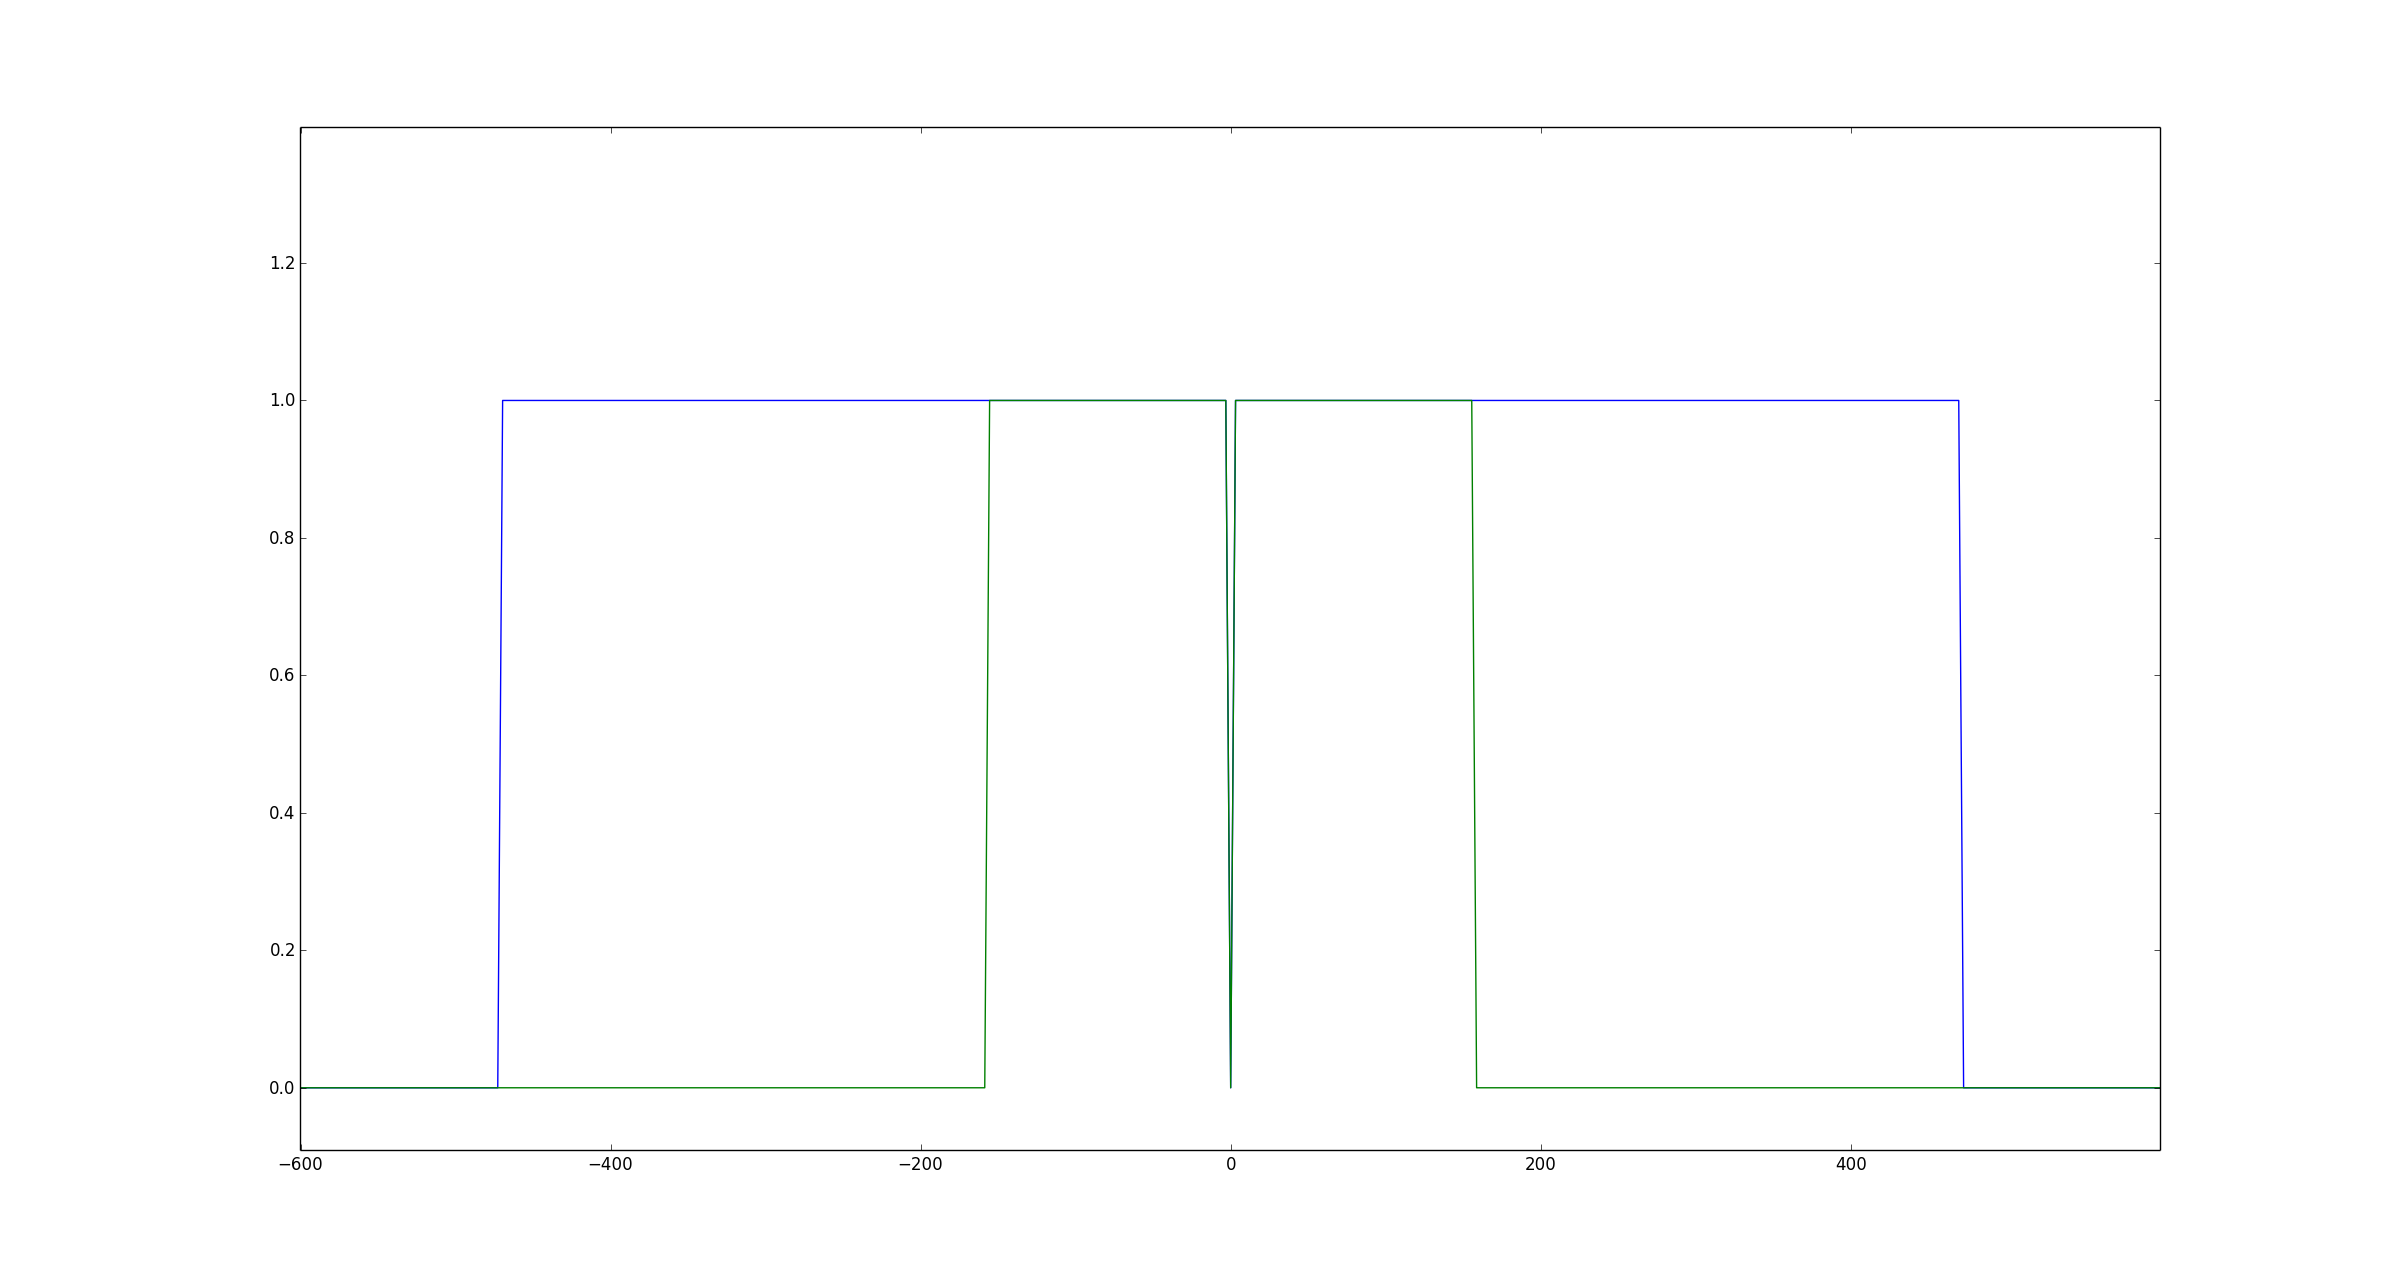
\includegraphics[width = 13.5cm]{images/Graf6.png}
              \vspace{-15px}
              \caption{Transformação de Fourier de $xc1 \textrm{(verde) e } yc1 \textrm{(azul)}$}
          \end{figure}
          \newpage
    \item \textbf{Q29:} O espectro que obtivemos provem dos processos de amostragem e de reconstrução de sinais. O método de amostragem consiste em obter um sinal formado por várias réplicas da transformada de $xc1$, réplicas estas que se vão repetindo com uma frequência pré-definida (frequência de amostragem). Posteriormente, efetua-se um escalamento de maneira a que o sinal se converta num sinal discreto.\\
          Neste caso, a condição do Teorema da Amostragem $(w_{s}>2w_{onda})$ não se verifica, o que leva ao chamado \textit{aliasing}, provocando diferenças no sinal à saída relativamente ao $xc1$ (Alguns troços do sinal desaparecem).\\
          No que toca à reconstrução de sinais, é possível afirmar que a frequência do sinal é modificada: frequência $yc1 =$ frequência $xc1$
          \begin{figure}[!ht]
              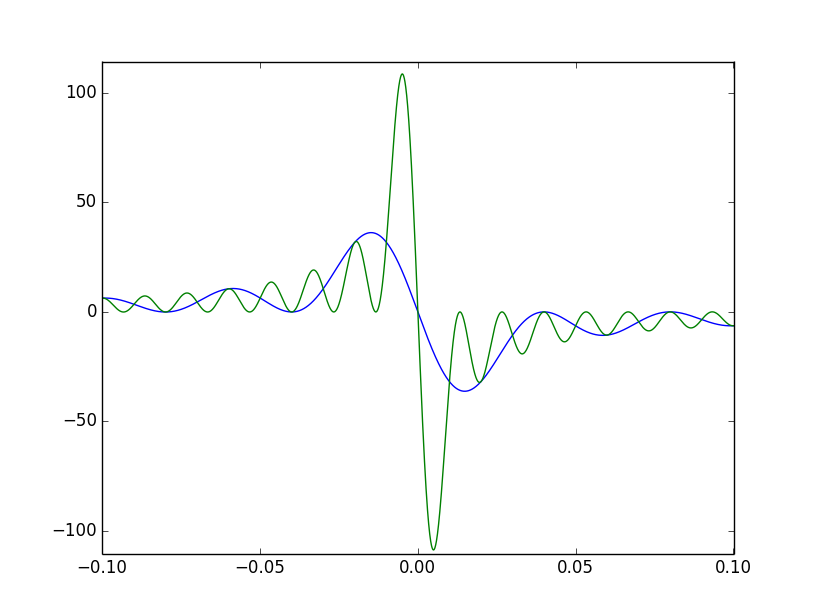
\includegraphics[width = 13.5cm]{images/Graf5.png}
              \vspace{-15px}
              \caption{Função $xc1 \textrm{(verde) e } yc1 \textrm{(azul)}$}
          \end{figure}
\end{itemize}
% % % % % % % % % % % % % % % % % % % % % % % % % % %
\end{document}